\section{Antenna Characteristics}
\label{sec:calibration}

In this section, the array's antenna gains are measured and then analyzed.
The measured antenna gains can then directly be employed as weights for the backprojection algorithm,
resulting in a calibrated array.
A subset of the extrated paramters can also be employed for offline calibration when using FFT-based imaging.


\subsection{Experiment Setup}
The experiment done to measure the array's antenna gain patterns was conducted outdoors.
This is preferable because the experiment requires more physical space than the previous stability analysis,
and of course minimal interfering clutter in that space.
As shown in \cref{fig:setup_rotating}, the sensor is mounted on a vertical rotating axis,
and a corner reflector is placed in front of the sensor.
Rotating the axis allows the sensor to observe the corner reflector from multiple angles, while retaining a fixed distance.
Doing this can be used to measure the antenna gains in azimuth;
to measure the antenna gains in elevation, the sensor is mounted on the same axis to rotate around its horizontal axis.
These two measurements are repeated for multiple reflector distances.

While the relative position of the rotating axis can be recorded with a decent resolution of around \SI{0.01}{\degree},
the absolute positioning of the reflector is hard to achieve with the same accuracy.
The sensor itself can however be used to improve positioning accuracy:
during setup, the phase of the peak caused by the reflector
is extracted with a similar method as in \cref{sec:stability_analysis} and displayed.
Mimimizing the phase differences between the array's channels by fine-tuning the reflector's position
ensures that it be located at boresight.
These measurements are repeated with multiple distances of the relector.\\
\begin{figure}[h]
  \centering
  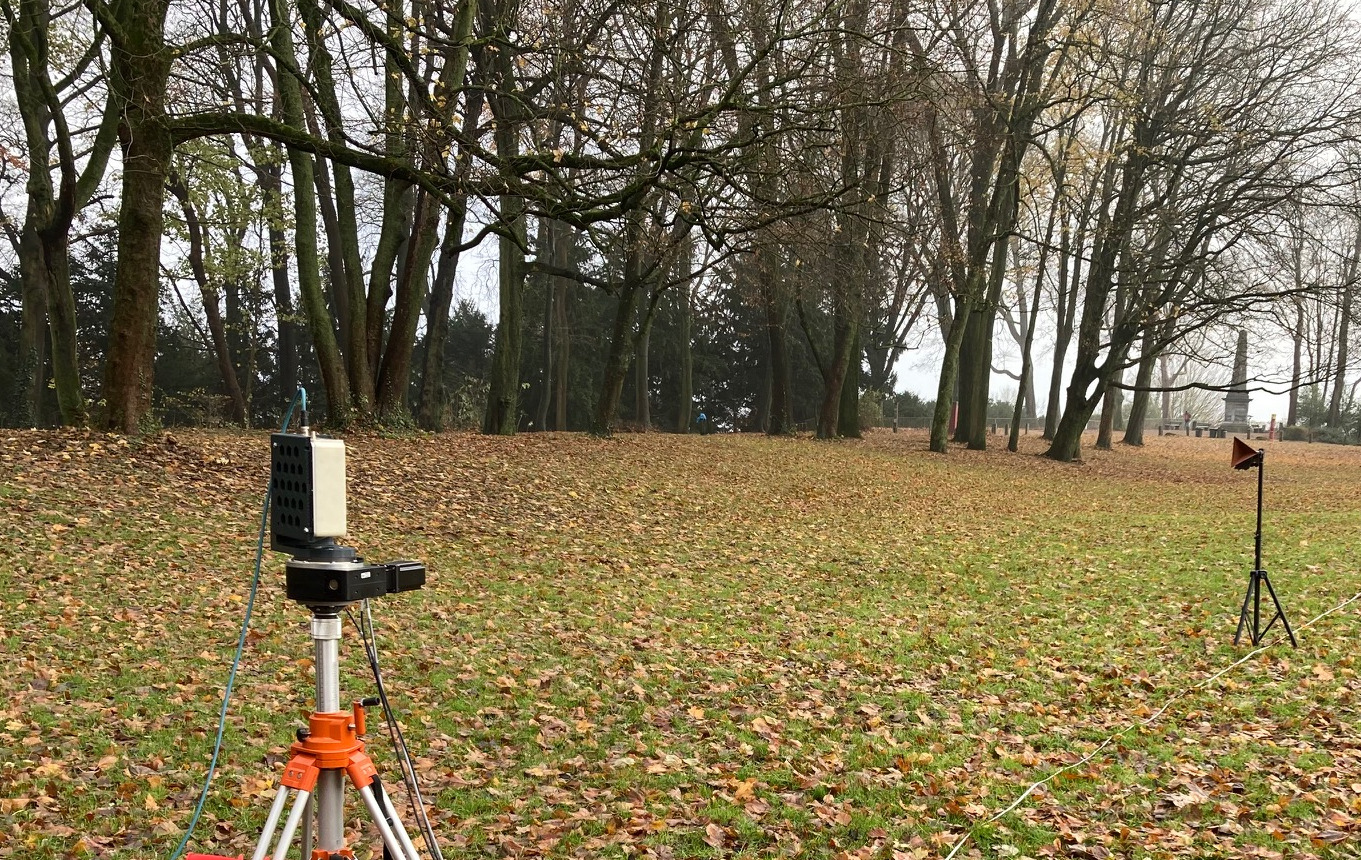
\includegraphics[width=0.6\textwidth]{../figures/setup_rotating.jpg}
  \caption{iMCR Antenna Gain Measurement Setup}
  \label{fig:setup_rotating}
\end{figure}

The field on which the experiment was set up is widely void of clutter, but not entirely.
Several trees and brushes are located at the edge of the scene.
Extra interference and reflections are caused by the floor.
It is also not perfectly level, varying in height by up to \SI{1}{\meter},
which means that the reflector is not always exactly at the same height.
The sensor mount also causes some problems [NEEDS DRAWING]:
when the sensor is mounted on its inside,
the rotational axis passes exactly through the antenna array's plane,
but some shading is occurs when the reflector is on the same side as the sensor mount's diagonal reinforcement.
When the sensor is mounted on the outside,
the rotational axis is no longer in the antenna array's plane,
adding complexity and inaccuracy to the subsequent analysis.

\subsection{Preprocessing and Analysis}
The objective of the subsequent analysis is to extract the antenna gains from the measured IF-signals.
In \cref{sec:single_channel_fmcw},
the the ideal deramped signal $y_{kl}[m]$ from channel $k$ at long-time index $l$
for a single reflector at position $\vec r_l$
is defined in \cref{eq:channel_gain} :
\begin{align*}
  y_{kl}[m] =  C_k(\vec r_l)e^{-j\omega_0\tau_{kl}}e^{-j\dot\omega\tau_{kl}mT_s}
\end{align*}
The square channel gain directly relates to the antenna gains $A_i$ and $B_j$
of the transmit antenna with index $i$ and the receive antenna with index $j$ that make up the channel:
\begin{align*}
  C_k^2 = \frac{P_{Rx}}{P_{Tx}}
  = G_{Tx}(\theta,\phi)  G_{Rx}(\theta,\phi) \frac{\sigma}{4\pi} \left(\frac{\lambda}{4\pi R_1 R_2}\right)^2
\end{align*}
For simplicity's sake, the following quantities are defined:
\begin{align}
  c_k(\theta,\phi) := \frac{C_k(r,\phi,\theta)}{\max |C_k(r,\phi,\theta)|}
\end{align}
will be called the \emph{channel characteristic}, and assumed to be constant in $r$ with $c_k(\theta,\phi) \in [0,1]$.
The \emph{antenna gains} are the relative maximum antenna gains of the transmit and receive antennas:
\begin{align}
  \underline A_i & :=  \frac{\max G_{Tx,i}(\theta,\phi)}{ G_{Rx,0}(\theta,\phi)}e^{j\psi_i}      \\
  \underline B_j & :=  \frac{\max G_{Rx,j}(\theta,\phi)}{ G_{Rx,0}(\theta,\phi)}e^{j\vartheta_j}
\end{align}
As defined in \cref{eq:kij}, each channel $k$ has a corresponding transmit antenna $i$ and a receive antenna $j$.
All antenna gains are defined with regards to the reference antenna, receive antenna 0.
They also include a phase offset which describe any mismatches in the individual antenna,
such as polarization, reflections in the antenna ports or length offsets in the transmission lines leading to them.

With that, the radar range equation can be rewritten as follows:
\begin{align*}
  \underline C_k^2 = \underline A_i \underline B_j c_k^2(\theta,\phi) e^{j2\left(\varphi_k-\omega_0\frac{R_1+R_2}{c_0}\right)}
  \frac{\sigma}{4\pi} \left(\frac{\lambda}{4\pi R_1 R_2}\right)^2
\end{align*}

The goal of the subsequent analysis is twofold:
to extract all parameters of the above signal model while identifying and removing interference through processing.

Limiting the analysis to a single range bin will work towards both reducing interference and extracting parameters:
ideally, the DFT spectrum of the IF signal consists of just a single peak,
weighted with the channel gain $C_k(\vec r)$ (see \cref{eq:y_fft}).
Thus, the channel gain can be extracted if the correct bin $\hat \Omega$ is picked:
\begin{align}
  \hat \Omega                                               & = \dot \omega \tau_k(\vec r_S)T_s              \\
                                                            & = \dot \omega \frac{R_1+R_2}{c}T_s             \\
  \Rightarrow \mathcal{F}_m\{y_k[m]\}(\Omega = \hat \Omega) & =    \underline C_k(\vec r_S) \label{eq:G_fft}
\end{align}

\subsection{Range Estimation}
\label{sec:range_est}


In order to improve the accuracy of the subsequent analysis, the exact position of the reflector is estimated from the radar data.
To do this, numerical optimization is employed to find the parameter set
$\hat R_s, \hat \theta_s, \hat \epsilon$ that minimizes the difference between
a range estimate $\hat R_{k,l}$ and the range spectral peak $R_{k,l}$ for all channels $k$ and recorded orientations $l$:
\begin{align}
  R_{k,l} = \arg \underset{r}{\max}\,\mathcal{F}_m\{y_{k,l}[m]\}\left(\Omega = \frac{N_{fft}r}{R_{max}}\right)
\end{align}

The range estimate $\hat R_{k,l}$ is determined geometrically from the distances of each channel's
transmit and receive antenna to the reflector. If the sensor is mounted to rotate in azimuth,
the range depends on the rotation angle $\theta_l $:

\begin{align}
  \hat R_{k,l}   & = \frac{\| \vec r_{TX,k} - \vec r_S(l) \|+\| \vec r_{RX,k} - \vec r_S(l) \|}{2}
  \\
  \vec{r}_{TX,k} & = \begin{bmatrix}
                       x_{TX,k} \\ y_{TX,k} \\ \hat \epsilon
                     \end{bmatrix},
  \vec r_{RX,k}       = \begin{bmatrix}
                          x_{RX,k} \\ y_{RX,k} \\ \hat \epsilon
                        \end{bmatrix},                                                                                        \\
  \vec r_S(l)    & = \begin{bmatrix}
                       (\hat R_S-\hat \epsilon) \text{sin}(\hat \theta_S-\theta_l) \\ 0 \\ (\hat R_S-\hat \epsilon) \text{cos}(\hat \theta_S-\theta_l)
                     \end{bmatrix},
\end{align}
If the sensor is mounted to rotate in its elevation, the reflector appears to move depending on the rotation in elevation $\phi$.
For a given rotation angle $\phi_l$, the reflector is located at
\begin{align}
  \vec r_S(l) & = \begin{bmatrix}
                    0 \\ (\hat R_S-\hat \epsilon) \text{sin}(\hat \phi_S-\phi_l) \\ (\hat R_S-\hat \epsilon) \text{cos}(\hat \phi_S-\phi_l)
                  \end{bmatrix},
\end{align}

In our setup, a signal is recorded with $\theta$ (or $\phi$, respectively) from \SIrange{0}{180}{\degree},
with the reflector located at roughly $R_S = \{2,8,18,32\}\si{\meter}$ and either $\theta_S = \SI{90}{\degree}$ or $\phi_S = \SI{90}{\degree}$. \\

With this, the loss $\mathcal L$ can be defined as the mean square difference between $\hat R$ and $R_{p}$,
the mean being computed as the average over all $K$ channels and $L$ sensor rotations:
\begin{align}
  \mathcal L(\hat R_s, \hat \theta_s, \hat \epsilon)
  = \frac{1}{KL}\sum_{l=0}^{L-1} \sum_{k=0}^{K-1} ( R_{k,l} - \hat  R_{k,l}(\hat R_s, \hat \theta_s, \hat \epsilon))^2
\end{align} \\

\begin{figure}[h]
  \centering
  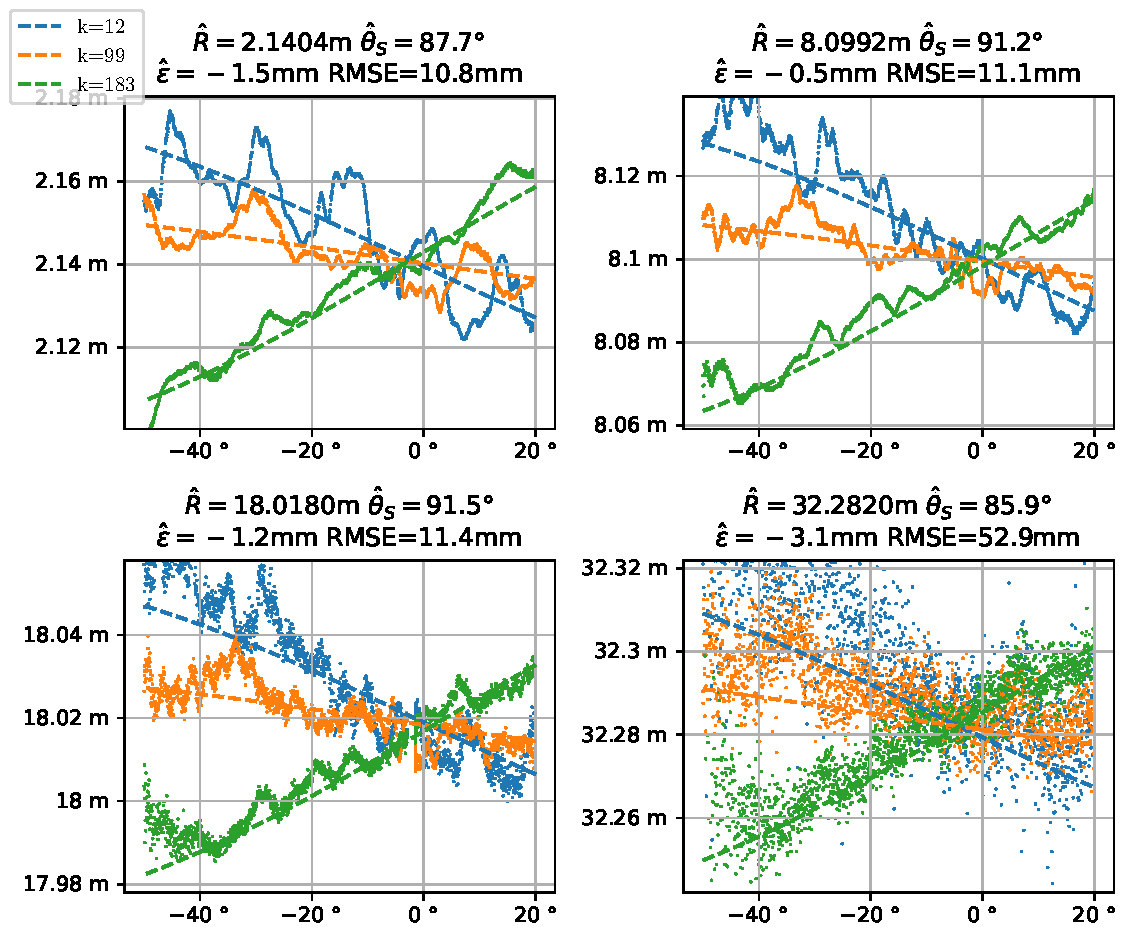
\includegraphics[width=\textwidth]{../figures/reflpos_estimate.pdf}
  \caption{Example Optimization Results}
  \label{fig:reflpos_estimate}
\end{figure}

\cref{fig:reflpos_estimate} shows the result of 100 iterations at an adaption rate of 0.05 at the example of three different channels,
comparing the measured spectral peaks (shown as points) to the estimated position (dotted line) of the reflector.
Only a subset of orientations is used for the estimate,
namely \SI{-50}{\degree} $<\theta_l-$\SI{90}{\degree}$<$ \SI{20}{\degree}. \\

For the first three measurements, the peak location oscillates around the estimate by \SIrange[range-units=single]{1}{2}{\cm}.
The \emph{root mean square error} (RMSE) is reduced to \SI{11}{\mm}.
Due to the decreasing signal level received from higher distances,
the fourth measurement has a higher relative noise level, resulting higher movement of the spectral peaks, and hence a much higher RMSE.

\newpage

\begin{figure}
  \centering
  \begin{subfigure}{\textwidth}
    \centering
    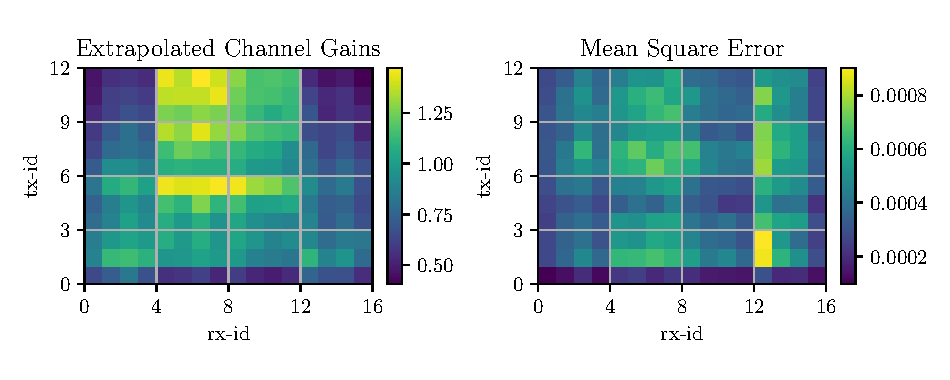
\includegraphics[width=\textwidth]{../figures/amplitude_linreg.pdf}
    \subcaption{Resulting Coefficents}
    \label{fig:amp_linreg}
  \end{subfigure}
  \vspace{1cm}
  \begin{subfigure}{0.5\textwidth}
    \centering
    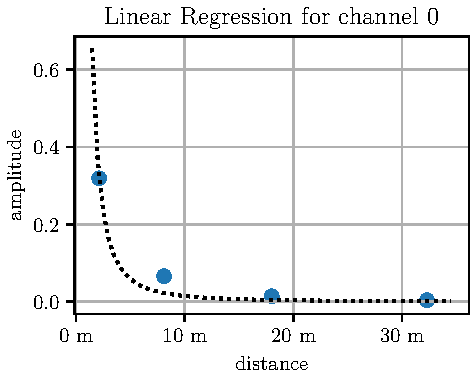
\includegraphics[width=\textwidth]{../figures/ch0_amplitude_linreg.pdf}
    \subcaption{Example: channel 0}
    \label{fig:ch0_amp_linreg}
  \end{subfigure}
  \caption{Linear Regression of Transmission Coefficients}
\end{figure}
\subsection{Amplitude}
\label{sec:amplitude}
First, the recorded amplitudes are analyzed, beginning with the influence of the angle of arrival.
To do this, each channel's range FFT spectrum's amplitude is evaluated at the respective calculated peak location $\hat \Omega$,
and then normalized by dividing it by its maximum.

The first parameters to extract are the three real-valued factors $A_i$, $B_j$ and $c(\theta,\phi)$.
First, we define a quantity that will be referrred to as the transmission coefficient:
\begin{align}
  \alpha_k = \sqrt{\frac{\sigma}{4\pi}A_iB_j}
\end{align}
Since the channel characteristic has been constrained to $[0,1]$,
the transmission constant can be expressed in terms of the two distances
$R_1 = \|\vec r_s - \vec r_{Tx,k}\|$ and $R_2 = \|\vec r_s - \vec r_{Rx,k}\|$, and other known constants: \\
\begin{align}
  \underset{\theta,\phi}{\text{max}} |\underline C_k(R,\theta,\phi)|
   & = \alpha_k\frac{\lambda}{4\pi R_1R_2} = \alpha_k \frac{1}{R_1R_2} \frac {2\pi c_0}{\omega}          \\
   & = \alpha_k \frac{1}{4\pi R_1R_2} \dfrac {2\pi c_0}{\omega_0 +  \dot \omega \frac{R_1+R_2}{c_0}}     \\
   & = \alpha_k \dfrac{c_0^2}{2R_1R_2\left(\omega_0c_0 +  \dot \omega (R_1+R_2)\right)} \label{eq:max_G}
\end{align}

With that, an estimate of the transmission coefficient $\hat \alpha_k$ can be obtained via linear regression.
An example linear regression is shown in \cref{fig:ch0_amp_linreg},
and the resulting estimates with their standard deviations are summarized in \cref{fig:amp_linreg}.

Having estimated the channel gains, we can now turn to analysing the channel characteristics.
Assuming the omptimal range bin $\hat \Omega$ is evaluated each time, we get
\begin{align*}
  \left|\mathcal{F}_m\{y_k[m]\}(\Omega = \hat \Omega)  \right| =  |C_k(\vec r)|
\end{align*}
Dividing that by the maximum gain (\ref{eq:max_G}) yields
\begin{align}
  \frac {|C_k(\vec r)|}{\underset{\theta,\phi}{\text{max}} |C_k(R,\theta,\phi)|}  = c_k(\theta,\phi)
\end{align}

\begin{figure}
  \centering
  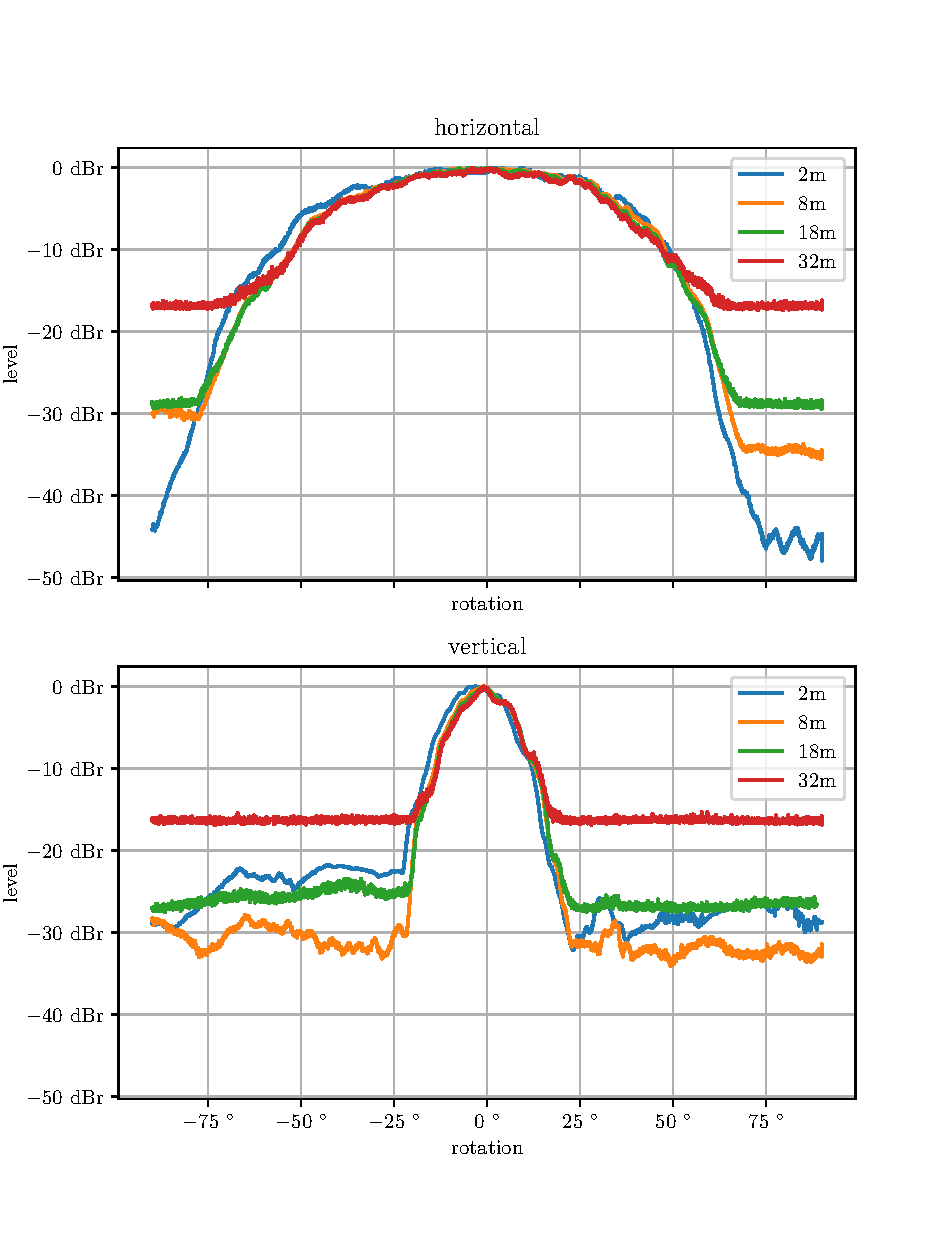
\includegraphics[width=\textwidth]{../figures/mean_amp.pdf}
  \caption{Mean Channel Characteristic for multiple reflector distances}
  \label{fig:mean_amp}
\end{figure}

\cref{fig:mean_amp} provides an overview by displaying the mean channel characteristic for each measurement.
It can be seen that the gain is strongest when the target is directly in boresight,
tapering off when the target is off-center. The reduction in gain is stronger when the target
moves off to the side in the elevation, than in azimuth. While the target remains stronger
than background noise up until an azimuth angle of around \SIrange{-75}{+75}{\degree},
it can only be seen in an elevation angle sector from \SIrange{-25}{+25}{\degree}.

The graphs of the horizontal measurements appear slightly asymmetrical, an effect which is investigated in the following.

\begin{figure}
  \centering
  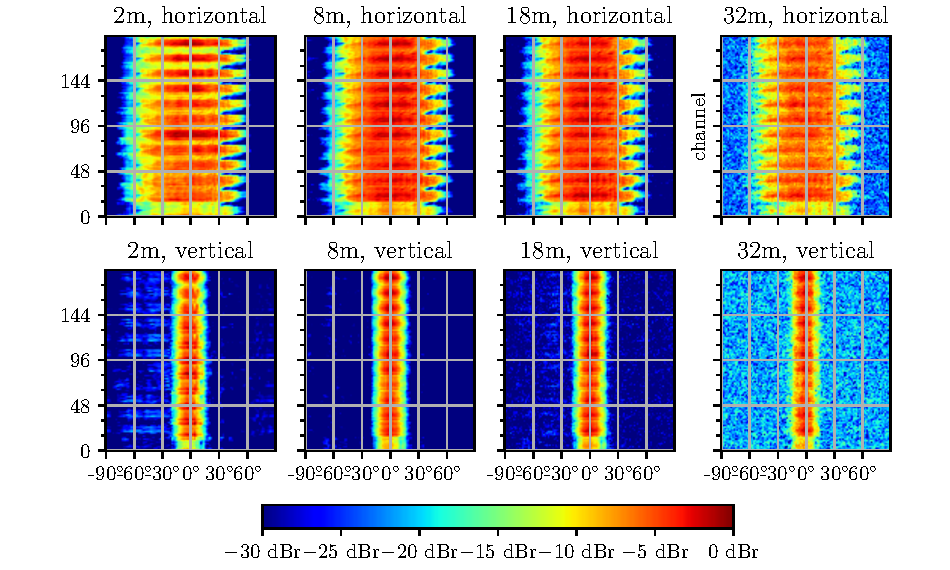
\includegraphics[width=\textwidth]{../figures/channel_amp.pdf}
  \caption{Channel-wise amplitude for multiple distances}
  \label{fig:chan_amp}
\end{figure}

A possible explanation for the asymmetry is the sensor mount,
which protrudes out on the right side of the array,
attenuating the signal received by antennas on that side when the reflector is behind said protrusion.

Investigating the individual channel gains (c.f. \ref{fig:chan_amp}) gives a first indication:
the asymmetry is most pronounced when comparing the range of \SIrange{30}{60}{\degree}
to its counterpart of \SIrange{-30}{-60}{\degree} for the horizontal measurements.
Namely, in the former range, the gain seems to oscillate every 16 channels.

\begin{figure}
  \centering
  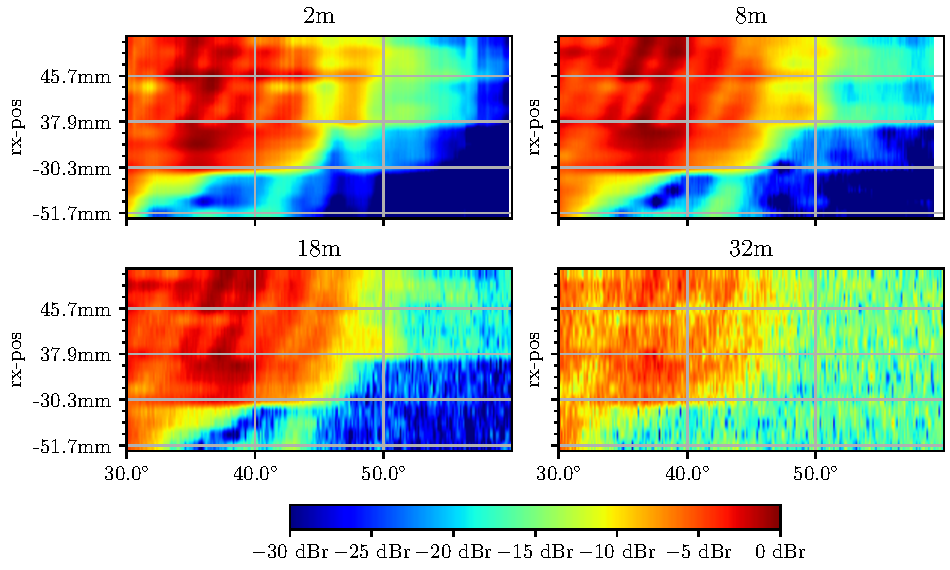
\includegraphics[width=\textwidth]{../figures/channel_amp_tx0.pdf}
  \caption{Channel-wise amplitude for multiple distances, channels arranged by Rx antenna position, only Tx antenna 0 active}
  \label{fig:chan_amp_tx0}
\end{figure}

To explore further, \cref{fig:chan_amp_tx0} zooms in on one period.
It shows the channel gain of the horizontal measurements for angles \SIrange{30}{60}{\degree}
of the channels in which transmit antenna 0 is active, arranged by the horizontal position of the receive antenna, from left to right.
It can now be seen that the channel gain of antennas closer to the sensor mount's protrusion drops
in amplitude at lower angles than that of the antennas further away from it,
confirming that the sensor mount is responsible for the asymmetry.
To get a more accurate estimate of the channel characteristics,
the measurements have to be repeated with the sensor mounted on the outside.\\

With this, the individual antenna gains and the channel characteristics have been extracted from the data.
In the next step, the recorded phases are analyzed. \\

\newpage
\subsection{Phase Estimation Techniques}

The first step in extracting the phase parameters from the recorded data is yet again
evaluating the signal's DFT phase at the optimum range bin $\hat \Omega = \frac{ N \dot \omega}{c_0 f_s}\hat R_k$,
which according to (\ref{eq:G_fft}) should ideally yield
\begin{align}
  \Phi_k(\vec r_S) :     & = \arg\, \mathcal{F}_m\{y_k[m]\} (\hat \Omega(\vec r_S)) \\
                         & =    \arg\,\underline C_k(\vec r_S)                      \\
                         & = \omega_0\tau_k(\vec r_S) + \varphi_k                   \\
  \text{with } \varphi_k & = \frac{\psi_{i}+\theta_{j}}{2}
  \text{ and } \tau_k    = \frac{2R_k}{c_0}
\end{align}

However, this part of the analysis is highly dependent on the accuracy of our assumptions,
specifically the distance between reflector and sensor.
The phase $\Phi_k(\theta) = \omega_0 \frac{2R_k(\theta)}{c_0} + \varphi_k$ changes immensely with small changes in said distance.

To illustrate, a change of $\Delta R_k = \SI{1}{\mm}$ would cause approximately the folowing phase shift:
\begin{align*}
  \Delta\Phi_k & = \omega_0 \frac{2\Delta R_k}{c_0}                                            \\
               & = 2\pi \cdot \SI{77e9}{\Hz} \cdot \frac{2\cdot\SI{1e-3}{\m}}{\SI{3e8}{\m/\s}} \\
               & = 0.5133 \pi = \SI{92.4}{\degree}
\end{align*}
The range estimate made in \cref{sec:range_est} had an RMSE of at least \SI{11}{\mm},
which introduces high uncertainty into the phase evaluation. \\

Another method to extract the phase from the recorded data is evaluating the FFT at the spectral peak,
which was the method of choice in \ref{sec:stability_analysis}.
Which method copes better with the presence of interference?
In the following, we will illustrate the effects of interference with a simulated signal,
as well as the impact of the interference on the two estimation methods accuracy.

Consider the signal received by an arbitray channel of the array $y(t,\theta)$.
Its frequency slowly changes as the orientation angle $\theta$;
for simplicity's sake, let the frequency shift linearly with $\omega(\theta)=2\pi (\SI{5}{\MHz} + \SI{1}{\MHz} \cdot \theta), \theta \in [-1,+3]$.
This results in our ideal signal
\begin{align*}
  y_{id}(t=mT_s,\theta) = 1 \cdot e^{-j\omega(\theta)mT_s}
\end{align*}
Introducing a source of interference with constant frequency $\omega_0$ and the amplitude $0.1$,
as well as a gaussian noise source $n(t,\theta) \sim \mathcal{N}(0;0.001)$, we get

\begin{align*}
  y(t=mT_s,\theta) = 1 \cdot e^{-j\omega(\theta)mT_s} + 0.1 \cdot e^{-j\omega_0 mT_s} + n(t,\theta)
\end{align*}

The spectrum of the ideal signal $Y_{id}(\Omega, \theta)$ and the degraded signal $Y(\Omega,\theta)$,
calculated with an $N=2048$ point FFT with $M=512$ samples in long-time, each corresponding to a different angle $\theta$,
is shown in fig. \ref{fig:interference_test_spectrum} in amplitude and phase.
\begin{figure}[h]
  \centering
  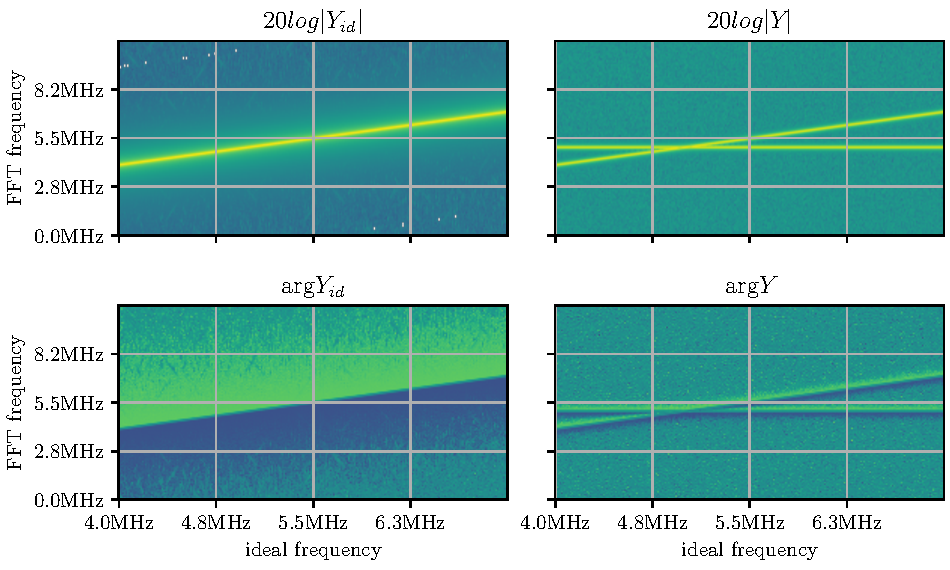
\includegraphics[width=\textwidth]{../figures/interference_test_fft.pdf}
  \caption{Spectra of example signal $Y$ and $Y_{id}$}
  \label{fig:interference_test_spectrum}
\end{figure}
The location of the both signals' spectral maxima can be seen in fig. \ref{fig:interference_test_peak},
showing that the interference causes the spectral maximum to move from its ideal location. \\
\begin{figure}
  \centering
  \begin{subfigure}{0.49\textwidth}
    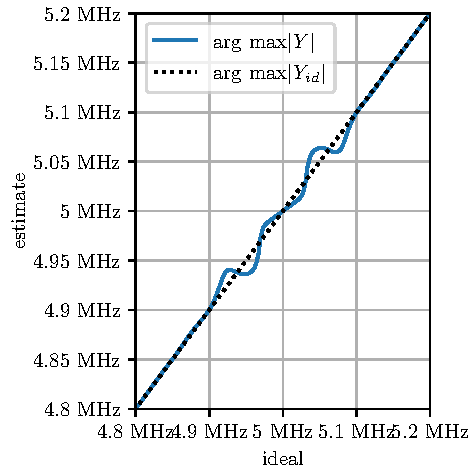
\includegraphics[width=\textwidth]{../figures/interference_test_peak.pdf}
    \subcaption{Peak Frequency}
    \label{fig:interference_test_peak}
  \end{subfigure}
  \hfill
  \begin{subfigure}{0.49\textwidth}
    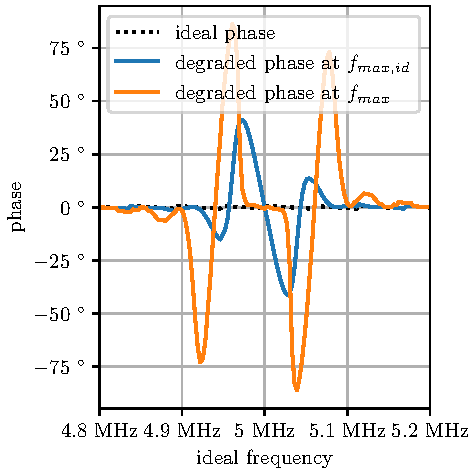
\includegraphics[width=\textwidth]{../figures/interference_peak_phase.pdf}
    \caption{Phase at peaks}
    \label{fig:interference_peak_phase}
  \end{subfigure}
  \caption{Extracting Phase from example spectra $Y$ and $Y_{id}$}
\end{figure}
\cref{fig:interference_peak_phase} finally shows the effect of interference on the phase.
We compare the phase of the ideal signal to phase of the degraded signal,
which is evaluated at both the ideal and the degraded signal's spectral maxima.
It can be seen that the latter method's phase diverges much more strongly from the ideal phase than that of the former,
and should therefor be preferred in the subsequent analysis. \\

\newpage
\subsection{Phase Analysis}
\label{sec:phase_analysis}
\begin{figure}
  \centering
  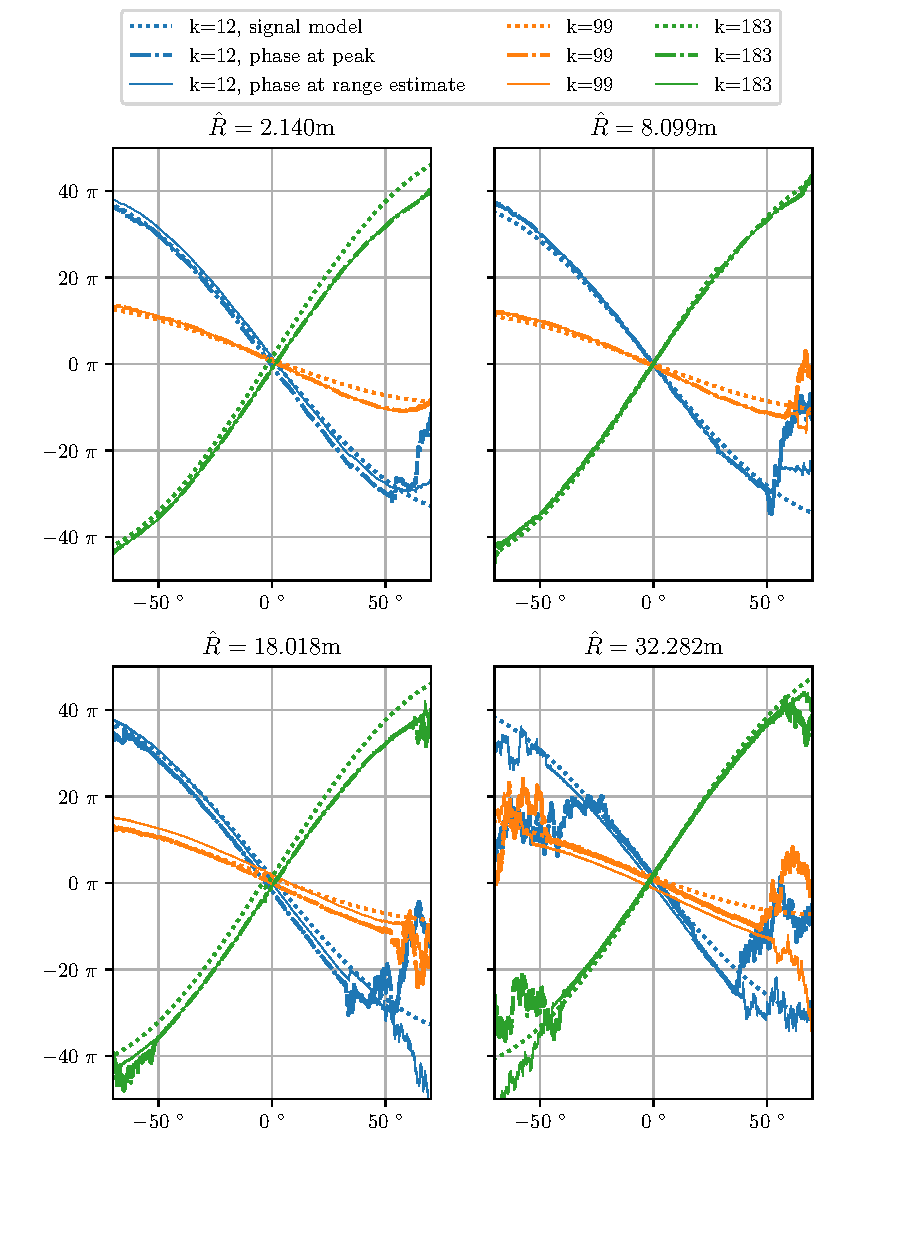
\includegraphics[width=\textwidth]{../figures/phase_estimates.pdf}
  \caption{Extracted Phase from measured signal, compared to signal model}
  \label{fig:measured_peak_phase}
\end{figure}
With knowledge of the robustness of our phase estimation against range estimation errors,
the task of extracting the phase parameters can be continued.
For better legibility of any graphs generated from the signal,
the phase of any given channel will be unwrapped from its original domain of $\theta \in [-\pi+\theta_s, \pi+\theta_s]$ such that no discontinuities
are visible when plotting phase against sensor orientation, while maintaining the original phase for $\theta = \theta_s$.

To assess the performance of the two techniques introduced in the previous section,
\cref{fig:measured_peak_phase} shows how they each compare to the signal model
\footnote{
  In this case, the signal model shown for comparison assumes that $\varphi_k = 0,\, \forall 0 \leq k<K$.
  Thus, the phase shown here is directly proportional to the estimated range $\hat R_k$:
  $$
    \hat\Phi_k(\theta) = \omega_0 \tau_k + 0 =  \frac{\omega_0}{c_0}2\hat R_k(\theta).
  $$
} for a few selected channels.
As it turns out, while being theoretically less robust against interference,
the phase evaluated at the signal peak is much smoother and matches our signal model much more closely. \\
\begin{figure}
  \centering
  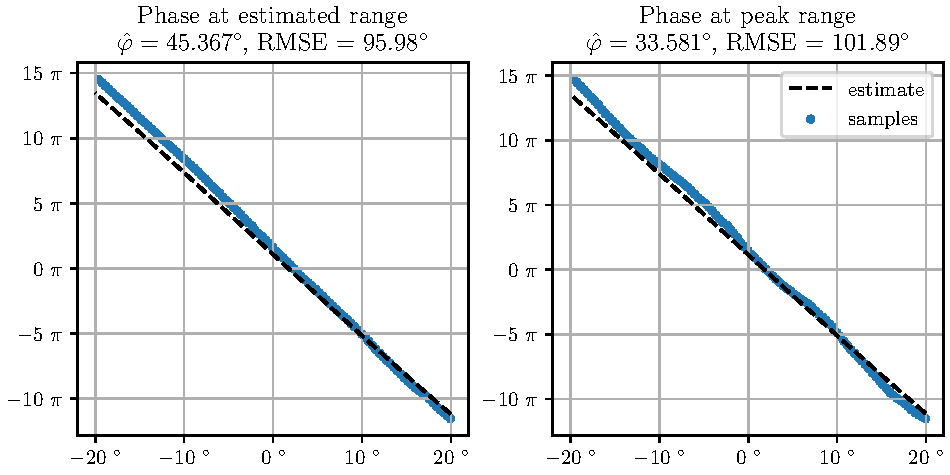
\includegraphics[width=\textwidth]{../figures/ch12_phase_linreg.pdf}
  \caption{Example: Channel 12 Phase Linear Regression}
  \label{fig:ch12_phase_linreg}
\end{figure}
Now, the channel phase offsets $\hat \varphi_k$ can be estimated using linear regression.
\cref{fig:ch12_phase_linreg} shows an example linear regression,
and the resulting channel phase offsets are shown in \cref{fig:phase_linreg}.
\begin{figure}
  \centering
  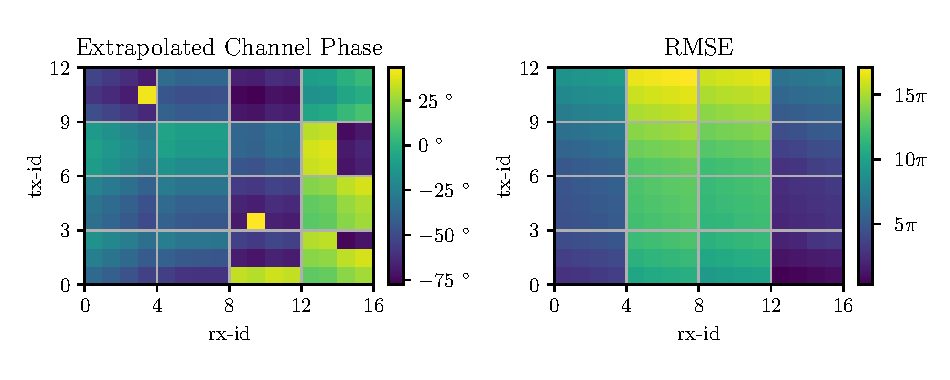
\includegraphics[width=\textwidth]{../figures/phase_linreg.pdf}
  \caption{Phase Linear Regression Overview}
  \label{fig:phase_linreg}
\end{figure}

\subsection{Antenna Separation}
To describe the array in terms of its channel gains is somewhat redundant.
As was defined in the underlying signal model, each channel gain $C_ke^{j\varphi_k}$ in actuality
just the product of the transmit and receive antenna gains, that is
\begin{align}
  C_k^2e^{j2\varphi_k} = A_i e^{j\psi_i} \cdot B_j e^{j\vartheta_j} \text{ for } k=N_{Tx}i+j
\end{align}

To more accurately describe the array,
the next step in our analysis is to estimate antenna gains of the receive and transmit array.
Multiple combinations were feasible, but the rightmost receive antenna 0 was defined as a reference antenna,
such that $B_0=1$ and $\vartheta_0 = 0$.

In the following, the channel gain amplitudes $\hat C_k$ that were estimated in \cref{sec:amplitude},
and the channel phase offsets $\hat \varphi_k$ from \cref{sec:phase_analysis}
are used to obtain estimates for the transmit and receive antenna parameters. \\

Thanks to the definition of a reference antenna,
the transmit antennas' amplitude and phase are easily obtained:
\begin{align}
  \hat A_i    & = \left.\hat C_k^2 \right|_{k=N_{Tx}i}     \\
  \hat \psi_i & = \left.\hat \varphi_k \right|_{k=N_{Tx}i}
\end{align}
With that, a least squares estimate for the remaining receive antennas' amplitude and phase is:
\begin{align}
  \hat B_{j\neq0}         & = \frac{1}{N_{Tx-1}} \sum_{i=1}^{N_{Tx-1}} \left. \frac{\hat C_k^2}{\hat A_i} \right|_{k=N_{Tx}i},        \\
  \hat \vartheta_{j\neq0} & = \frac{1}{N_{Tx-1}} \sum_{i=1}^{N_{Tx-1}} \left. \frac{2\hat \varphi_k}{\hat \psi_i} \right|_{k=N_{Tx}i}
\end{align}
The resulting antenna parameters are shown in tables \ref{tab:tx_gains} and \ref{tab:tx_gains}.
\begin{table}[h]
  \centering
  \begin{subtable}[t]{0.4\textwidth}
    \begin{tabular}{ccc}
      \toprule
      \textbf{Antenna} & \textbf{Gain}   & \textbf{Phase} \\
      \midrule
      0                & \num{4.134e+06} & 53.596°        \\
      1                & \num{7.847e+06} & 125.805°       \\
      2                & \num{7.363e+06} & 48.354°        \\
      3                & \num{6.169e+06} & -126.556°      \\
      4                & \num{5.445e+06} & -13.976°       \\
      5                & \num{6.815e+06} & -111.434°      \\
      6                & \num{5.174e+06} & -81.855°       \\
      7                & \num{3.962e+06} & 82.760°        \\
      8                & \num{3.517e+06} & 119.322°       \\
      9                & \num{2.831e+06} & 1.485°         \\
      10               & \num{2.291e+06} & 7.703°         \\
      11               & \num{2.158e+06} & -53.846°       \\
      \bottomrule
    \end{tabular}
    \subcaption{Tx Antennas}
    \label{tab:tx_gains}
  \end{subtable}
  \hfill
  \begin{subtable}[t]{0.4\textwidth}
    \begin{tabular}{ccc}
      \toprule
      \textbf{Antenna} & \textbf{Gain} & \textbf{Phase} \\
      \midrule
      0                & \num{1.000}   & 0.000°         \\
      1                & \num{1.463}   & -7.095°        \\
      2                & \num{1.676}   & -26.095°       \\
      3                & \num{1.426}   & 0.712°         \\
      4                & \num{3.797}   & -1.052°        \\
      5                & \num{3.635}   & 26.672°        \\
      6                & \num{3.999}   & 42.318°        \\
      7                & \num{3.703}   & -2.503°        \\
      8                & \num{3.391}   & 49.492°        \\
      9                & \num{2.867}   & -2.698°        \\
      10               & \num{2.751}   & 69.663°        \\
      11               & \num{2.631}   & -40.625°       \\
      12               & \num{1.393}   & 8.481°         \\
      13               & \num{0.987}   & -11.289°       \\
      14               & \num{1.129}   & -1.515°        \\
      15               & \num{0.820}   & -5.109°        \\
      \bottomrule
    \end{tabular}
    \subcaption{Rx Antenna Gains}
    \label{tab:rx_gains}
  \end{subtable}
  \caption{Estimated Antenna Parameters with Reference Rx0}
\end{table}

\subsection{Conclusion}
In this section, a method for estimating the antenna gains from real-world antenna measurements has been formulated
that optimizes the estimation's accuracy and robustness against interference.
The summarized steps are as follows:
\begin{enumerate}
  \item Setup the reflector in front of the sensor.
        For each distance to measure, center the reflector by observing a live readout of the phase at the spectral peak caused by the reflector,
        and positioning the sensor such that the phase differences between channels is minimal.
  \item From the measurements, extract the range of the spectral peak caused by the reflector for each channel and sensor orientation.
        Use numerical optimization to find a set of model parameters ($\hat R_s$, $\hat \theta_s$ or $\hat \phi_s$, and $\hat\epsilon$)
        that best matches the spectral peaks.
  \item Evaluate the amplitude of the spectrum at the frequency corresponding to the estimated range from the previous step.
        The maximum amplitude across all angles is the channel gain $C_k / R^2$,
        and the remaining attenuation is the channel characteristic $\hat c_k(\theta,\phi) \in [0,1]$.
        With linear regression across all measured distances, the channel gain at \SI{1}{\m} can be estimated.
        The estimated channel chararacteristic $\hat c_k(\theta,\phi)$ can indicate orientations with low SNR and/or high interference.
  \item Evaluate the phase of the spectrum at the frequency corresponding to the estimated range.
        Unwrap the phase of each channel such that the phase for $\theta = \hat \theta_s$ is in $[-\pi,\pi]$.
        Find the channel phase offset $\varphi_k$ that best matches the signal model to the measured phase.
  \item Separate each square channel gain $\hat C_k^2e^{j2\hat \varphi_k}$ into a transmit gain $A_i e^{j\psi_i}$ and a receive gain $B_j e^{j\vartheta_j}$.
        Do this by defining a receive antenna as a reference.
\end{enumerate}

Following these steps gives a decent estimate of the systems's physical properties with relatively lax requirements on the measurement itself.
This is especially desirable since \cref{sec:stability_analysis} demonstrated a need for frequent in-field calibration,
since the system parameters may change after restarting, and also shift over time. \\

More sophisticated methodology is required to achieve accurate measurements of the system.
Controlling the positioning of the reflector relative to the sensor more closely,
for example by placing the reflector on a linear axis,would greatly improve accuracy.

Interference sources in the environment would also have to be reduced.
This would involve moving the experiment to a more controlled environment,
such as a low-reflection room.

Another area of improvement lies in channel separation.
Since the reference antenna in the described method is not external,
but rather a part of the system under test,
all the results of our analysis indicate are relative differences between antennas.
Instead, an external antenna with known characteristics could replace the reflector,
allowing for more accurate measurements of the individual antennas' absolute characteristics.



